\subsection{Newton's Method}\label{ssec:newton}

In this section, we propose\todojames{our main?} 
a simple and powerful method to solve~(\ref{eq:bcd:block-update}).
By solving the sub-gradient problem of~(\ref{eq:bcd:block-update}),
we see that the solution $\beta^\star$ must satisfy
\begin{align}
    \beta
    &=
    \begin{cases}
    \pr{\Sigma + \frac{\lambda}{\norm{\beta}_2} I}^{-1} v ,& \norm{v}_2 > \lambda \\
    0 ,& \norm{v}_2 \leq \lambda
    \end{cases}
    \label{eq:newton:block-solution}
\end{align}
Without loss of generality, we consider the first case when $\beta^\star \neq 0$.
Without knowing $\norm{\beta^\star}_2$, there is no closed-form solution for $\beta^\star$.
In an endeavor to find an expression for $\norm{\beta^\star}_2$,
we take the $\ell_2$ norm on both sides to get that $\norm{\beta^\star}_2$ must satisfy
\begin{align}
    \sum\limits_{i=1}^p
    \frac{v_i^2}{(\Sigma_{ii} \norm{\beta}_2 + \lambda)^2}
    =
    1
    \label{eq:newton:norm-solution}
\end{align}
Unfortunately, there is no closed-form solution for~(\ref{eq:newton:norm-solution}) either.
However, we will shortly see that a simple Newton's Method 
can numerically solve~(\ref{eq:newton:norm-solution}) efficiently with guaranteed convergence.
In turn, once we find $\norm{\beta^\star}_2$, we may substitute it
into~(\ref{eq:newton:block-solution}) to get the full solution $\beta^\star$ in $O(p)$ time.
We note in passing that~(\ref{eq:newton:block-solution}) and~(\ref{eq:newton:norm-solution})
were previously discovered~\citep{sls:2016},
however, there is no mention of how to quickly solve for $\beta^\star$ or $\norm{\beta^\star}_2$.

We now discuss how to solve~(\ref{eq:newton:norm-solution}).
First, define $\varphi : [0, \infty) \to \R$ by
\begin{align}
    \varphi(h)
    &:=
    \sum\limits_{i=1}^p
    \frac{v_i^2}{(\Sigma_{ii} h + \lambda)^2}
    - 1
    \label{eq:varphi-def}
\end{align}
so that~(\ref{eq:newton:norm-solution}) is now a root-finding problem for $\varphi$.
In~\Cref{appendix:properties-varphi}, we show that $\varphi$ is 
convex and is, without loss of generality, 
strictly decreasing with a unique root.
By standard convex analysis, Newton's Method guarantees convergence to the root of $\varphi$
for any initial point $h^{(0)}$ (see~\Cref{appendix:newton-convergence}).
\Cref{alg:newton:newton} summarizes Newton's Method.

\begin{algorithm}[t]
    \caption{Newton's Method}\label{alg:newton:newton}
    \KwData{$\Sigma$, $v$, $\lambda$, $\varepsilon$, $h^{(0)}$}
    $h \gets h^{(0)}$\;
    \While{$\abs{\varphi(h)} > \varepsilon$} {
        $h \gets h - \frac{\varphi(h)}{\varphi'(h)}$\;
    }
    return $h$\;
\end{algorithm}

Since $\varphi$ is strongly convex with Lipschitz second derivative,
we also have quadratic convergence and each iteration costs $O(p)$~\citep{boyd:2004}.
In principle, our setting is one of the best settings for Newton's Method to succeed.
While FISTA 
%(\Cref{alg:pgd:fista}) 
and the adaptive restarted version
%(\Cref{alg:pgd:fista-adares}) 
also give the same convergence rate~\citep{beck:2009,odonoghue:2015},
\Cref{fig:newton:pgd-newton} shows a clear improvement for Newton's Method in practice.
Here, accuracy was measured as
\begin{align}
    &\max\limits_{i=1,\ldots,p} 
    \abs{\hat{\beta}_i - \beta_i}
    \label{eq:accuracy}
    \\
    &\hat{\beta} 
    :=
    \text{ solution from algorithm}
    \nonumber
    \\
    &\beta
    :=
    \pr{\Sigma + \frac{\lambda}{\norm{\hat{\beta}}_2} I}^{-1} v
    \nonumber
\end{align}
Note that the PGD methods fail to converge as $p$ increases,
and even when they converge, Newton's Method performs 10 to 1000 times faster.
One very important benefit of Newton's Method 
is that the optimization domain remains one-dimensional \emph{regardless of the input dimension $p$}.
However, the PGD methods directly optimize in $\R^p$,
so their instability grows with increasing $p$ due to the curse of dimensionality.
As a result, the speed and convergence stability in Newton's Method 
makes it the more desirable algorithm.

\begin{figure}[t]
    \centering
    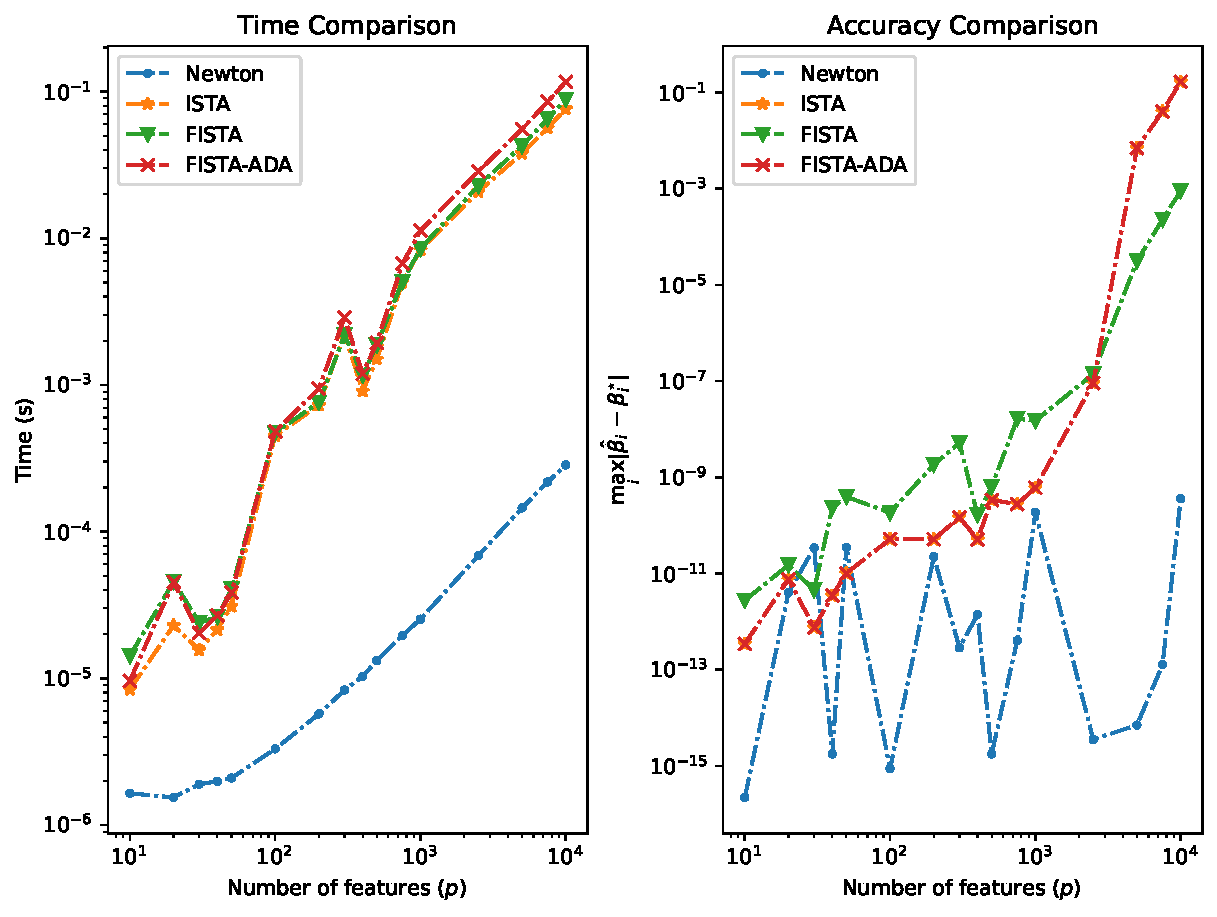
\includegraphics[width=0.7\textwidth]{figures/pgd_newton_fista_newton.pdf}
    \caption{Time and accuracy comparison between the PGD methods 
    in~\Cref{ssec:pgd} and Newton's Method.
    Overall, the PGD methods suffer from large computational overhead due to large number of iterations,
    and fails to converge as the dimension $p$ increases.
    Contrastingly, Newton's Method is quite stable, properly converges, and runs 10 to 1000 times faster.
    }
    \label{fig:newton:pgd-newton}
\end{figure}

It is widely known that descent methods including Newton's Method
is highly sensitive to the initialization.
A poor initialization may lead to slow convergence
while an initialization close to the root will be rewarded with incredible convergence speed
(see~\Cref{fig:newton-abs:stuck}).
The question that remains is: how to choose the initial starting point $h^{(0)}$?
%Despite the convergence guarantee irrespective of the choice of $h^{(0)}$,
%it is nonetheless ideal to choose an initial point close to the root for an even faster convergence.
We recommend selecting any $h^{(0)}$ such that $\varphi(h^{(0)}) \geq 0$.
For example, $h^{(0)} \equiv 0$ is sufficient since by definition $\varphi(0) > 0$.
If $h^{(0)}$ is such that $\varphi(h^{(0)}) < 0$,
then it is possible that $h^{(1)} < 0$.
In fact, due to the flat tail of $\varphi$, it is extremely common for $h^{(1)}$ to be negative.
In this case, after projecting back to $[0, \infty)$ (i.e. setting $h^{(1)} = 0$),
we arrive at the same sequence as if we had started with $h^{(0)} = 0$.
For this reason, it is almost always better to 
set the initial point such that $\varphi(h^{(0)}) \geq 0$.
Although $h^{(0)} = 0$ is a valid choice, it may also lead to large number of iterations,
especially if $\lambda$ is small
(see~\Cref{fig:bench:newton-compare}).
In~\Cref{ssec:newton-abs}, we describe our most performant and robust 
modification to the vanilla Newton's Method that reduces iterations in nearly all cases.
